\documentclass{beamer}
%\usetheme{Warsaw}
\usepackage[utf8]{inputenc}
\usepackage{minted}
\usepackage{fancyvrb}
\usepackage{xspace}
\newcommand{\myurl}[1]{\href{#1}{\texttt{#1}}}
\newcommand{\email}[1]{\href{mailto:#1}{\texttt{#1}}}

\title[mpi4py]{MPI for Python}
\subtitle{\myurl{http://mpi4py.scipy.org}}
\author[L.~Dalcin]{Lisandro~Dalcin~\\\email{dalcinl@gmail.com}}
\institute[]
{
  Numerical Porous Media Center\\
  Computer, Electrical, and Mathematical Sciences \& Engineering\\
  King Abdullah University of Science and Technology\\
  Thuwal, Saudi Arabia\\
  -\\
  Centro de Investigación de Métodos Computacionales \\
  Consejo Nacional de Investigaciones Científicas y Técnicas\\
  Santa Fe, Argentina
}
\date [ACM-Python-Tut '14]
{
  ACM Student Chapter Python Tutorials\\
  KAUST, Saudi Arabia\\
  February, 2014
}

\AtBeginSection[]
{
  \begin{frame}
    \tableofcontents[currentsection]
  \end{frame}
}

\newcommand{\Cpp}{C\protect\raisebox{.18ex}{++}\xspace}

\begin{document}

\begin{frame}
  \titlepage
\end{frame}

\section*{Outline}
\begin{frame}
  \frametitle{Outline}
  \tableofcontents
\end{frame}

% --- Overview ---

\section{Overview}

\begin{frame}
  \frametitle{What is \textbf{mpi4py}?}
  \begin{itemize}
  \item Python bindings for \href{http://www.mpi-forum.org}{\textbf{MPI}},
    (\emph {Message Passing Interface}).
  \item API based on the standard MPI-2 \Cpp bindings.
  \item Almost all MPI calls are supported.
    \begin{itemize}
    \item targeted to MPI-2 implementations.
    \item also works with old MPI-1 implementations.
    \item in-development: full support for MPI-3.
    \end{itemize}
  \end{itemize}
\end{frame}

%% \begin{frame}
%%   \frametitle{Implementation}
%%   Implemented with \href{http://www.cython.org}{\textbf{Cython}}
%%   \begin{itemize}
%%   \item Code base far easier to write, maintain, and extend.
%%   \item Faster than other solutions (mixed Python and C codes).
%%   \item A \textsl{pythonic} API that runs at C speed !
%%   \end{itemize}
%% \end{frame}
%% 
%% \begin{frame}
%%   \frametitle{Implementation - Cython [1]}
%%   \footnotesize
%%   \inputminted[firstline=1]{cython}{cython-mpi4py.pxi}
%% \end{frame}
%% 
%% \begin{frame}
%%   \frametitle{Implementation - Cython [2]}
%%   \footnotesize
%%   \inputminted[firstline=3]{cython}{cython-mpi4py.pyx}
%% \end{frame}

\begin{frame}
  \frametitle{Features -- MPI-1}
  \begin{itemize}
  \item Process groups and communication domains.
    \begin{itemize}
    \item intracommunicators
    \item intercommunicators
    \end{itemize}
  \item Point to point communication.
    \begin{itemize}
    \item blocking (send/recv)
    \item nonblocking (isend/irecv + test/wait)
    \end{itemize}
  \item Collective operations.
    \begin{itemize}
    \item Synchronization (barrier)
    \item Communication (broadcast, scatter/gather)
    \item Global reductions (reduce, scan)
    \end{itemize}
  \end{itemize}
\end{frame}

\begin{frame}
  \frametitle{Features -- MPI-2}
  \begin{itemize}
  \item Extended collective operations.
  \item Dynamic process management (spawn, connect/accept).
  \item Parallel I/O (read/write).
  \item One sided operations, a.k.a. RMA (put/get/accumulate).
  \end{itemize}
\end{frame}

\begin{frame}
  \frametitle{Features -- Python}
  \begin{itemize}
  \item Communication of Python objects.
    \begin{itemize}
    \item high level and very convenient, based in \texttt{pickle}
      serialization
    \item can be slow for large data (CPU and memory consuming)
    \end{itemize}
    \fbox{\texttt{send(object)}}\\
    \fbox{%
      \texttt{object} $\longrightarrow{}$%
      \texttt{pickle.dump()} $\longrightarrow{}$%
      \texttt{MPI\_Send()}
    }
    \\\hspace{39ex}\\
    \fbox{\texttt{object = recv()}}
    \fbox{%
      \texttt{object} $\longleftarrow{}$%
      \texttt{pickle.load()} $\longleftarrow{}$%
      \texttt{MPI\_Recv()}}
  \item Communication of array data
    (e.g. \href{http://numpy.scipy.org}{\textbf{NumPy}} arrays).
    \begin{itemize}
    \item lower level, slightly more verbose
    \item very fast, almost C speed (for messages above 5-10 KB)
    \end{itemize}
    \fbox{message = \texttt{[object, (count, displ), datatype]}}
  \end{itemize}
\end{frame}

\begin{frame}
  \begin{center}
    Point to Point Throughput -- Gigabit Ethernet
  \end{center}
  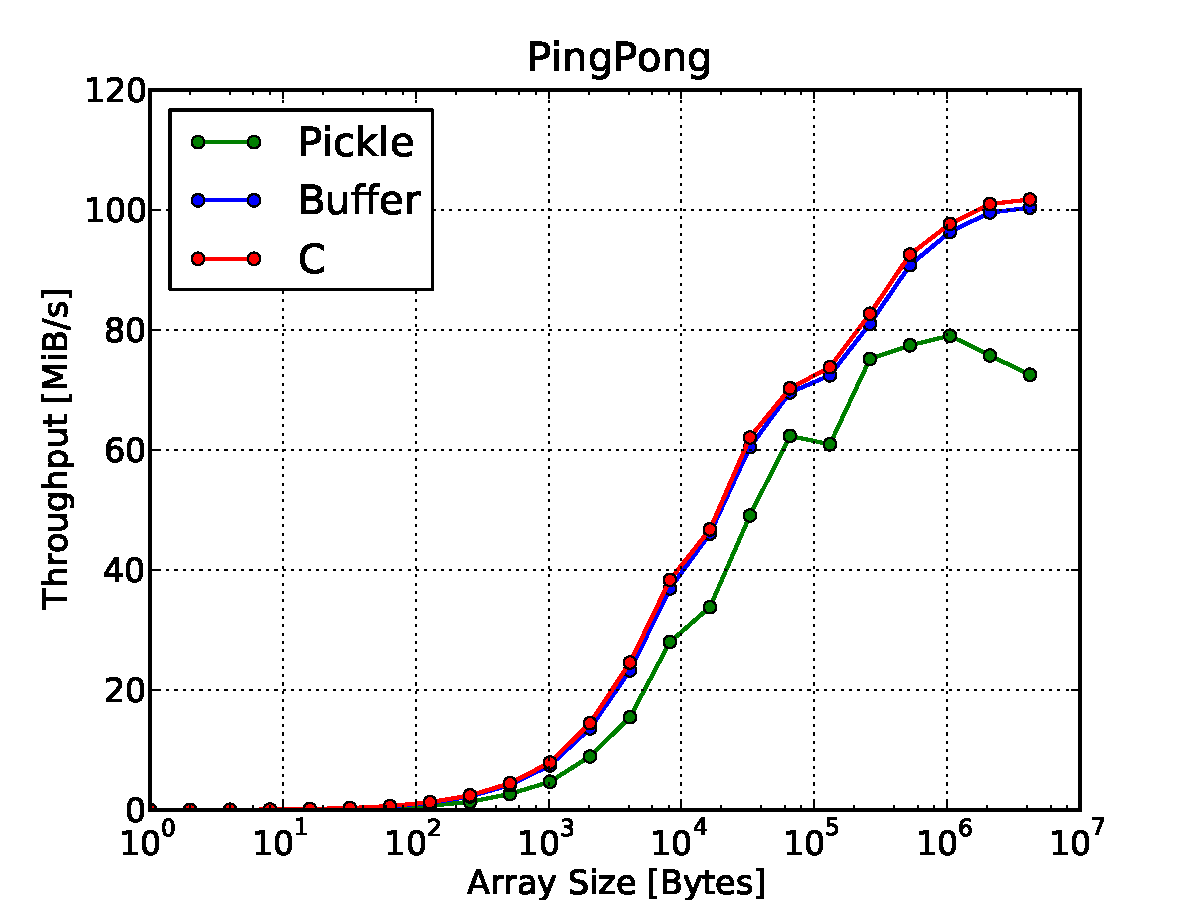
\includegraphics[scale=0.5]{PingPong_GE.pdf}
\end{frame}
\begin{frame}
  \begin{center}
    Point to Point Throughput -- Shared Memory
  \end{center}
  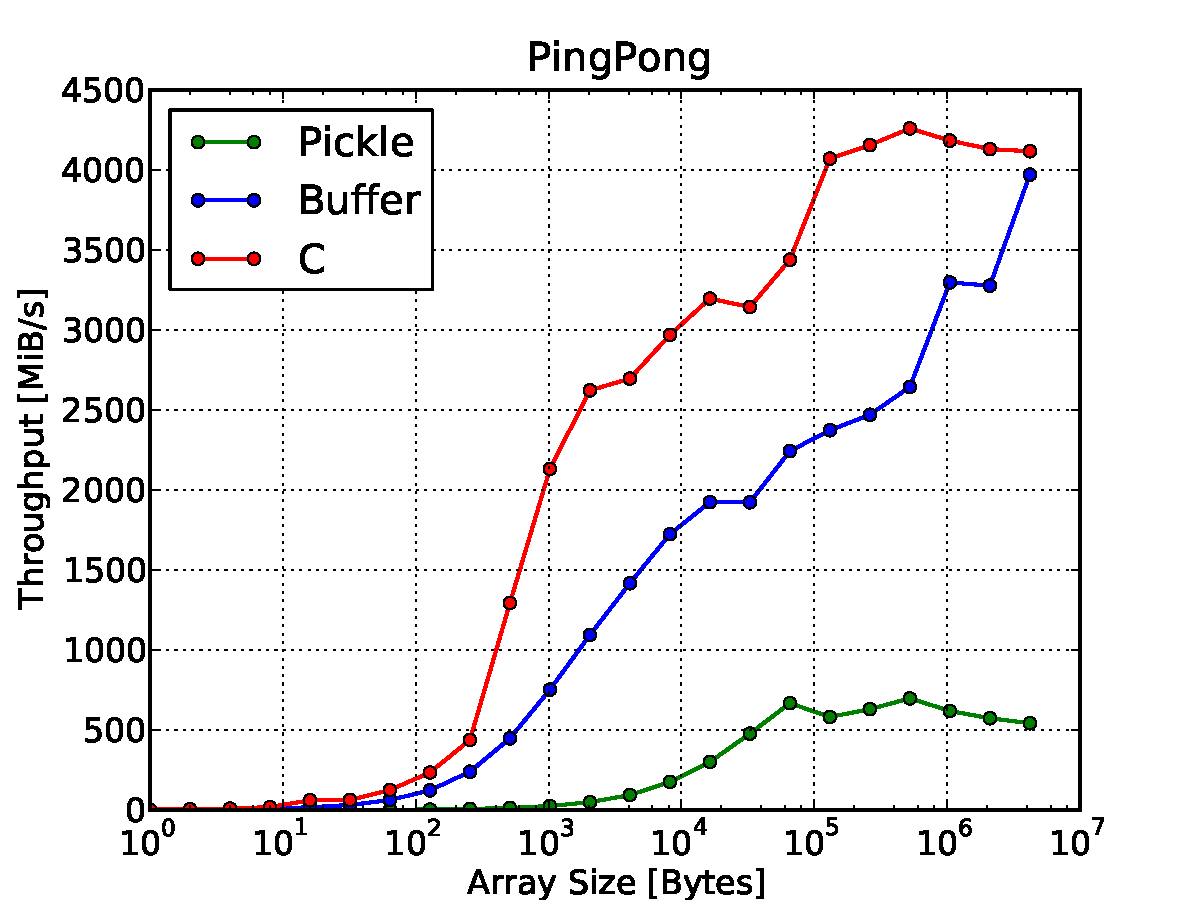
\includegraphics[scale=0.5]{PingPong_SM.pdf}
\end{frame}

%% \begin{frame}
%%   \frametitle{Features -- Interoperability}
%%   Good support for wrapping other MPI-based codes.
%%   \begin{itemize}
%%   \item You can use \href{http://cython.org}{\textbf{Cython}}
%%     (\texttt{cimport} statement).
%%   \item You can use \href{http://swig.org}{\textbf{SWIG}}
%%     (\textsl{typemaps} provided).
%%   \item You can use \href{http://f2py.com}{\textbf{F2Py}}
%%     (\texttt{py2f()}/\texttt{f2py()} methods).
%%   \item You can use
%%     \href{http://www.boost.org}{\textbf{Boost::Python}} or
%%     \textbf{hand-written C} extensions.
%%   \end{itemize}
%%   \textbf{mpi4py} allows you to use any
%%   MPI-based C/\Cpp/Fortran library from Python.
%% \end{frame}


\begin{frame}[fragile]
  \frametitle{Features -- IPython}
  Integration with \href{http://ipython.scipy.org}{\textbf{IPython}}
  enables MPI to be used \emph{interactively}.
  \begin{itemize}
  \item Start engines with MPI enabled
\begin{verbatim}
   $ ipcluster start -n 16 --engines=MPI
\end{verbatim}
  \item Connect to the engines
\begin{verbatim}
   $ ipython
   In [1]: from IPython.parallel import Client
   In [2]: rc = Client()
   In [3]: view = rc[:]
   In [4]: view.activate()
\end{verbatim}
  \item Execute commands using \texttt{\%px}
\begin{verbatim}
   In [5]: %pxconfig --block
   In [6]: %px from mpi4py import MPI
   In [7]: %px print(MPI.Get_processor_name())
\end{verbatim}
  \end{itemize}
\end{frame}

% --- Hello World! ---

\section{Hello World!}

\begin{frame}[fragile]
  \frametitle{Hello World! -- C}
  \inputminted[linenos]{c}{helloworld.c}
\end{frame}

\begin{frame}[fragile]
  \frametitle{Hello World! -- Fortran 90}
  \inputminted[linenos]{fortran}{helloworld.f90}
\end{frame}

\begin{frame}[fragile]
  \frametitle{Hello World! -- \Cpp}
  \inputminted[linenos]{cpp}{helloworld.cxx}
\end{frame}

\begin{frame}[fragile]
  \frametitle{Hello World! -- Python}
  \inputminted[linenos]{python}{helloworld.py}
  \begin{block}{}
\begin{verbatim}
$ mpiexec -n 4 python helloworld.py
Hello, World! I am process 0 of 4 on localhost
Hello, World! I am process 1 of 4 on localhost
Hello, World! I am process 2 of 4 on localhost
Hello, World! I am process 3 of 4 on localhost
\end{verbatim}
  \end{block}
\end{frame}

\begin{frame}
  \frametitle{Exercise \#0}
  \begin{enumerate}[a)]
  \item Compile and run the C/Fortran/\Cpp version of \emph{Hello, World!}.
  \item Run the Python version of \emph{Hello, World!}.
  \item Use \textbf{mpi4py} interactively with \textbf{IPython}.
  \end{enumerate}
\end{frame}

% --- Point to Point ---

\section{Point to Point Communication}

\begin{frame}[fragile]
  \begin{itemize}
  \item Blocking communication
    \begin{itemize}
    \item Python objects
      {\footnotesize
\begin{verbatim}
comm.send(obj, dest=0, tag=0)
obj = comm.recv(None, src=0, tag=0)
\end{verbatim}
      }
    \item Array data
      {\footnotesize
\begin{verbatim}
comm.Send([array, count, datatype], dest=0, tag=0)
comm.Recv([array, count, datatype], src=0, tag=0)
\end{verbatim}
      }
    \end{itemize}
  \item Nonblocking communication
    \begin{itemize}
    \item Python objects
      {\footnotesize
\begin{verbatim}
request = comm.isend(object, dest=0, tag=0)}
request.Wait()
\end{verbatim}
      }
    \item Array data
      {\footnotesize
\begin{verbatim}
req1 = comm.Isend([array, count, datatype], dest=0, tag=0)
req2 = comm.Irecv([array, count, datatype], src=0, tag=0)
MPI.Request.Waitall([req1, req2])}
\end{verbatim}
      }
    \end{itemize}
  \end{itemize}
\end{frame}

\begin{frame}
  \frametitle{PingPong}
  \inputminted[linenos]{python}{p2p_pingpong.py}
\end{frame}

\begin{frame}
  \frametitle{PingPing}
  \inputminted[linenos]{python}{p2p_pingping.py}
\end{frame}

\begin{frame}
  \frametitle{Exchange}
  \inputminted[linenos]{python}{p2p_exchange.py}
\end{frame}

\begin{frame}
  \frametitle{PingPing with NumPy arrays}
  \inputminted[linenos]{python}{p2p_pingping-numpy.py}
\end{frame}

\begin{frame}
  \frametitle{Exercise \#1}
  \begin{enumerate}[a)]
  \item Modify the \emph{PingPong} example to communicate NumPy arrays.\\
    \textbf{Tip}: use \texttt{Comm.Send()} and \texttt{Comm.Recv()}
  \item Modify the \emph{Exchange} example to communicate NumPy arrays.\\
    Use nonblocking communication for both sending and receiving.\\
    \textbf{Tip}: use \texttt{Comm.Isend()} and \texttt{Comm.Irecv()}
  \end{enumerate}
\end{frame}

% --- Collectives ---

\section{Collective Operations}

\begin{frame}
  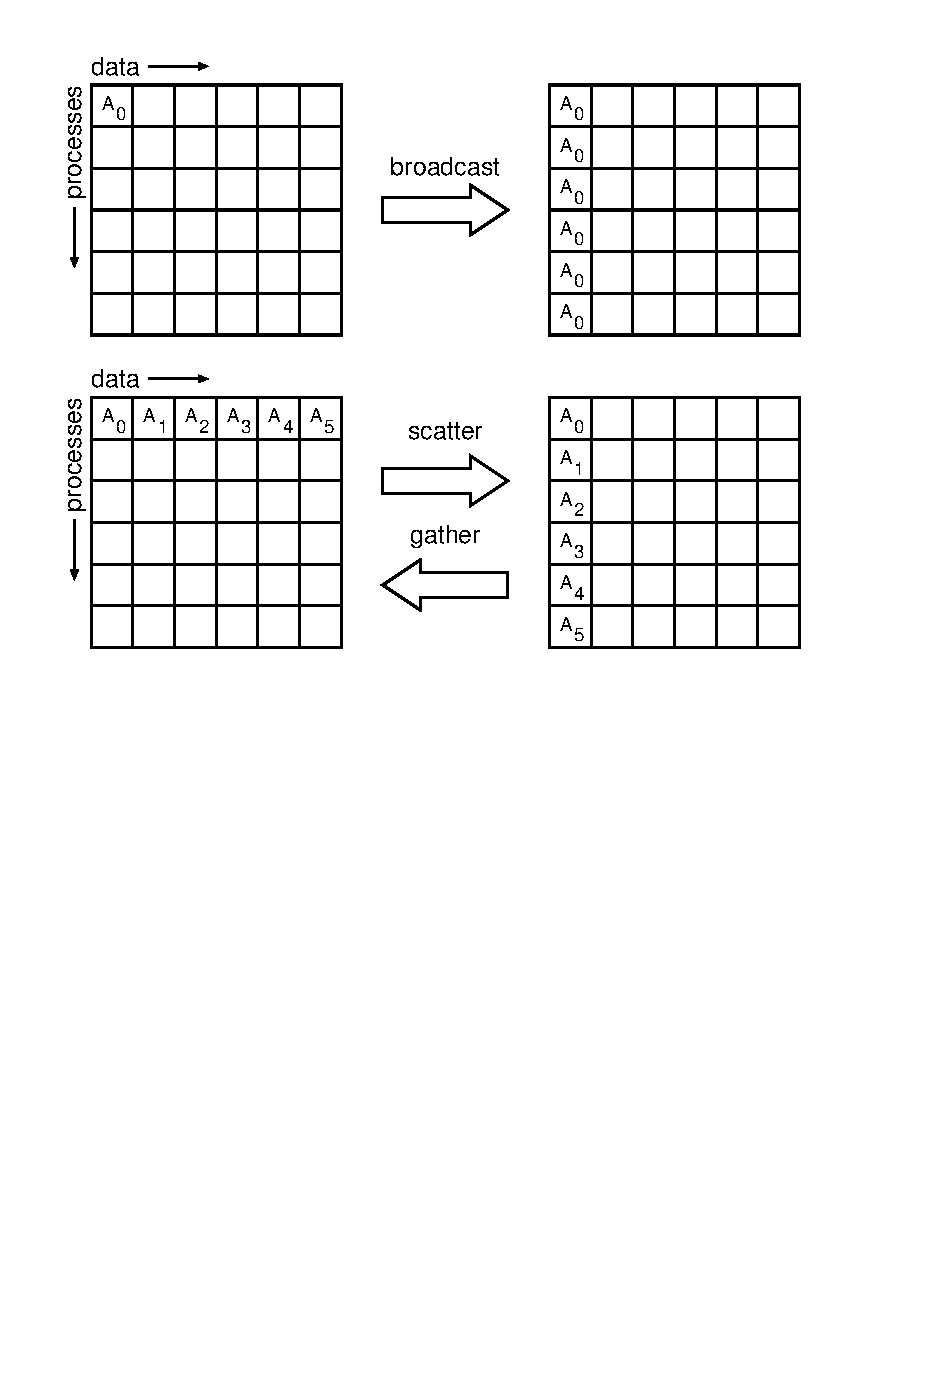
\includegraphics[scale=0.75]{collectives1.pdf}
\end{frame}

\begin{frame}
  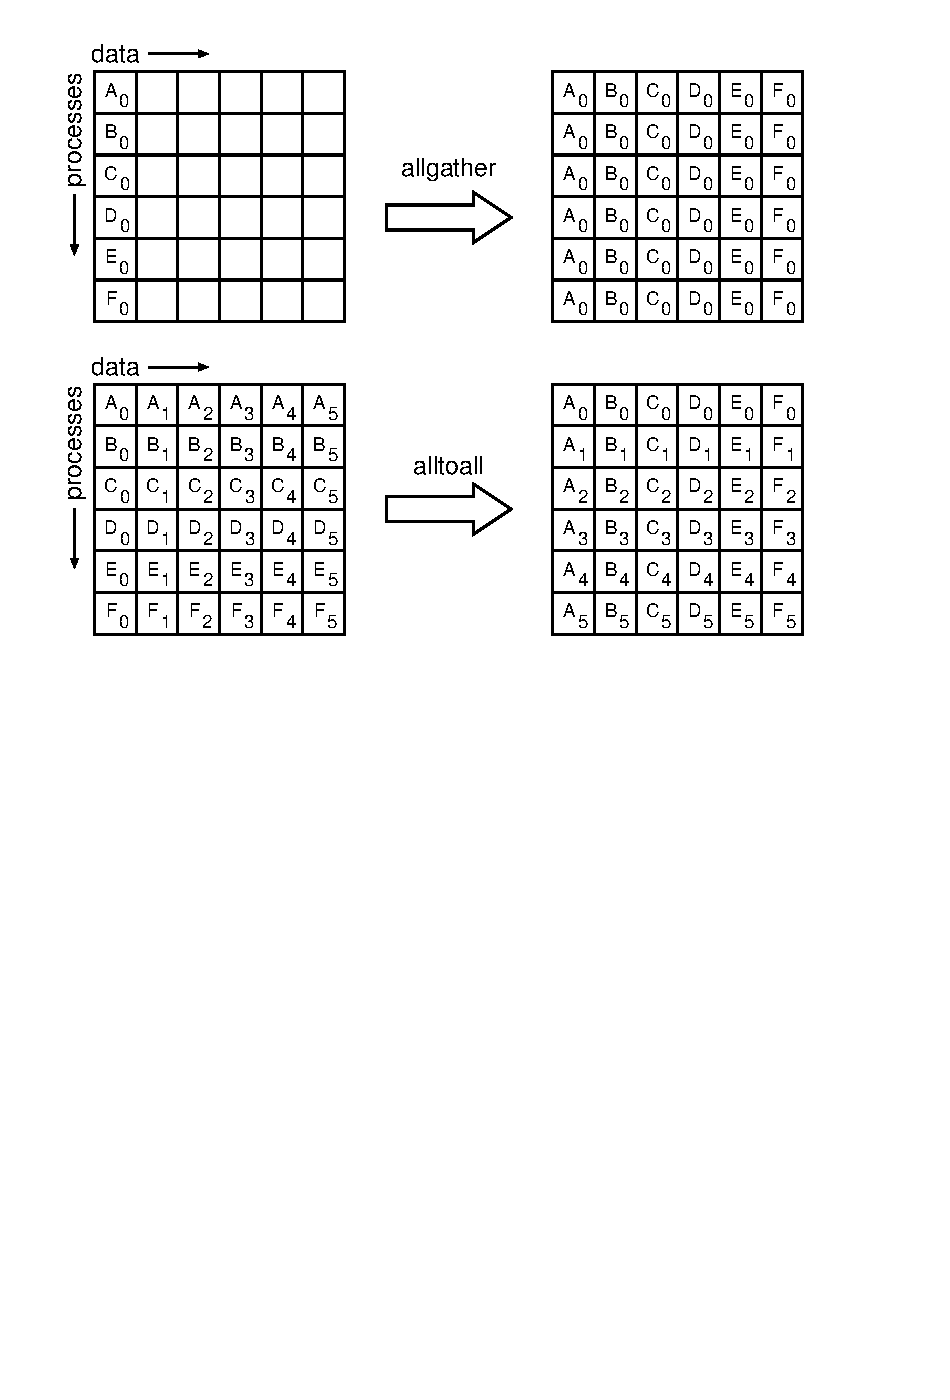
\includegraphics[scale=0.75]{collectives2.pdf}
\end{frame}

\begin{frame}
  \frametitle{Broadcast}
  \inputminted[linenos]{python}{coll_bcast.py}
\end{frame}

\begin{frame}
  \frametitle{Scatter}
  \inputminted[linenos]{python}{coll_scatter.py}
\end{frame}

\begin{frame}
  \frametitle{Gather \& Gather to All}
  \inputminted[linenos]{python}{coll_gather.py}
\end{frame}

\begin{frame}
  \frametitle{Reduce \& Reduce to All}
  \inputminted[linenos]{python}{coll_reduce.py}
\end{frame}

\begin{frame}
  \frametitle{Exercise \#2}
  \begin{enumerate}[a)]
  \item Modify the \emph{Broadcast}, \emph{Scatter}, and \emph{Gather}
    examples to communicate NumPy arrays.
  \item Write a routine implementing parallel
    \emph{matrix}--\emph{vector} product
    \texttt{y~=~matvec(comm,A,x)}.
    \begin{itemize}
    \item the global matrix is dense and square.
    \item matrix rows and vector entries have matching block
      distribution.
    \item all processes own the same number of matrix rows.
    \end{itemize}
    \textbf{Tip}: use \texttt{Comm.Allgather()} and \texttt{numpy.dot()}
  \end{enumerate}
\end{frame}

% --- Compute Pi ---

\section{Compute Pi}

\begin{frame}
  \frametitle{Compute Pi}
  \Large
  \begin{equation*}
    \pi =
    \int_0^1 \frac{4}{1+x^2} dx \approx
    \frac{1}{n}\sum_{i=0}^{n-1}\frac{4}{1+(\frac{i+0.5}{n})^2}
  \end{equation*}
\end{frame}

\begin{frame}[t]
  \frametitle{Compute Pi -- sequential}
  \inputminted[linenos]{python}{compute_pi-seq.py}
\end{frame}

\begin{frame}[t]
  \frametitle{Compute Pi -- parallel [1]}
  \inputminted[linenos,firstline=1,lastline=14]{python}
  {compute_pi-mpi.py}
\end{frame}

\begin{frame}[t]
  \frametitle{Compute Pi -- parallel [2]}
  \inputminted[linenos,firstline=16]{python}
  {compute_pi-mpi.py}
\end{frame}

\begin{frame}
  \frametitle{Exercise \#3}
  Modify \emph{Compute Pi} example to employ NumPy.\\
  \smallskip\smallskip
  \textbf{Tip}: you can convert a Python \texttt{int}/\texttt{float}
  object to a NumPy \emph{scalar} with \texttt{x~=~numpy.array(x)}.
\end{frame}

%% % --- Mandelbrot ---
%% 
%% \section{Mandelbrot Set}
%% 
%% \begin{frame}
%%   \frametitle{Mandelbrot Set}
%%   
\includegraphics[scale=0.5]{mandelbrot.pdf}
%% \end{frame}
%% 
%% \begin{frame}[t]
%%   \frametitle{Mandelbrot Set -- sequential [1]}
%%   \inputminted[linenos,firstline=1,lastline=13]{python}
%%   {mandelbrot-seq.py}
%% \end{frame}
%% 
%% \begin{frame}[t]
%%   \frametitle{Mandelbrot Set -- sequential [2]}
%%   \inputminted[linenos,firstline=15]{python}
%%   {mandelbrot-seq.py}
%% \end{frame}
%% 
%% \begin{frame}
%%   \frametitle{Mandelbrot Set -- partitioning}
%%   \begin{minipage}{\textwidth}
%%     \centering
%%     
\includegraphics[scale=0.25]{mandelbrot.pdf}
%%   \end{minipage}
%%   \begin{columns}[t]
%%     \begin{column}{0.45\textwidth}
%%       \centering
%%       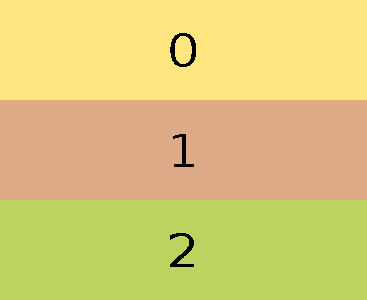
\includegraphics[scale=0.5]{dist-block.pdf}\\
%%       Block distribution
%%     \end{column}
%%     \begin{column}{0.45\textwidth}
%%       \centering
%%       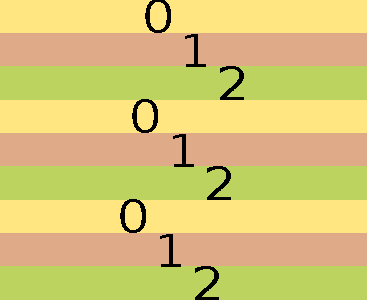
\includegraphics[scale=0.5]{dist-cyclic.pdf}\\
%%       Cyclic distribution
%%     \end{column}
%%   \end{columns}
%% \end{frame}
%% 
%% \begin{frame}[t]
%%   \frametitle{Mandelbrot Set -- parallel, block [1]}
%%   \inputminted[linenos,firstline=1,lastline=13]{python}
%%   {mandelbrot-mpi-block.py}
%% \end{frame}
%% \begin{frame}[t]
%%   \frametitle{Mandelbrot Set -- parallel, block [2]}
%%   \inputminted[linenos,firstline=15,lastline=29]{python}
%%   {mandelbrot-mpi-block.py}
%% \end{frame}
%% \begin{frame}[t]
%%   \frametitle{Mandelbrot Set -- parallel, block [3]}
%%   \inputminted[linenos,firstline=31,lastline=39]{python}
%%   {mandelbrot-mpi-block.py}
%% \end{frame}
%% \begin{frame}[t]
%%   \frametitle{Mandelbrot Set -- parallel, block [4]}
%%   \inputminted[linenos,firstline=41,lastline=55]{python}
%%   {mandelbrot-mpi-block.py}
%% \end{frame}
%% \begin{frame}[t]
%%   \frametitle{Mandelbrot Set -- parallel, block [5]}
%%   \inputminted[linenos,firstline=57,lastline=62]{python}
%%   {mandelbrot-mpi-block.py}
%% \end{frame}
%% 
%% \begin{frame}
%%   \frametitle{Exercise \#4}%
%%   Measure the wall clock time $T_i$ of local computations at each
%%   process for the \emph{Mandelbrot Set} example with \textbf{block} and
%%   \textbf{cyclic} row distributions.\\
%%   What is the best row distribution regarding load balancing?\\
%%   \smallskip\smallskip
%%   \textbf{Tip}: use \texttt{Wtime()} to measure wall time, compute
%%   the ratio $T_\text{max}/T_\text{min}$ to compare load balancing.
%% \end{frame}


%% % --- DynProc ---
%% 
%% \section{Dynamic Process Management}
%% 
%% \begin{frame}
%%   \frametitle{Dynamic Process Management}
%%   \begin{itemize}
%%   \item Useful in assembling complex distributed applications. Can
%%     couple \textbf{independent parallel codes} written in
%%     \textbf{different languages}.
%%   \item Create new processes from a running program.\\
%%     -- \texttt{Comm.Spawn()} and \texttt{Comm.Get\_parent()}
%%   \item Connect two running applications together.\\
%%     -- \texttt{Comm.Connect()} and \texttt{Comm.Accept()}
%%   \end{itemize}
%% \end{frame}
%% 
%% \begin{frame}
%%   \frametitle{Dynamic Process Management -- Spawning} Spawning new
%%   processes is a \emph{collective operation} that creates an
%%   \textbf{intercommunicator}.
%%   \begin{itemize}
%%   \item Local group is group of spawning processes (parent).
%%   \item Remote group is group of new processes (child).
%%   \item \texttt{Comm.Spawn()} lets parent processes spawn the child
%%     processes. It returns a new intercommunicator.
%%   \item \texttt{Comm.Get\_parent()} lets child processes find
%%     intercommunicator to the parent group. Child processes have own
%%     \texttt{COMM\_WORLD}.
%%   \item \texttt{Comm.Disconnect()} ends the parent--child
%%     connection. After that, both groups can continue running.
%%   \end{itemize}
%% \end{frame}
%% 
%% \begin{frame}[t]
%%   \frametitle{Dynamic Process Management -- Compute Pi (parent)}
%%   \small\inputminted[linenos]{python}{compute_pi-parent.py}
%% \end{frame}
%% 
%% \begin{frame}[t]
%%   \frametitle{Dynamic Process Management -- Compute Pi (child)}
%%   \small\inputminted[linenos]{python}{compute_pi-child.py}
%% \end{frame}
%% 
%% \begin{frame}
%%   \frametitle{Exercise \#5}
%%   \begin{enumerate}[a)]
%%   \item Implement the \emph{Compute Pi} \textbf{child} code in
%%     \textbf{C} or \textbf{\Cpp}. Adjust the parent code in Python to
%%     spawn the new implementation.
%%   \item Compute and plot the \emph{Mandelbrot Set} using spawning with
%%     parent/child codes implemented in Python.\\
%%     \textbf{Tip}: Reuse the provided parent code in Python and
%%     translate the child code in Fortran 90 to Python.
%%   \end{enumerate}
%% \end{frame}


% --- Closing ---

\section*{Closing}

\begin{frame}
  \Large
  Do not hesitate to ask for help \ldots \par
  \begin{itemize}
  \item Mailing List: \url{mpi4py@googlegroups.com}
  \item Mail\&Chat:   \url{dalcinl@gmail.com}
  \end{itemize}
  \bigskip
  \begin{centering}
   \Huge Thanks!\par
  \end{centering}
\end{frame}

\end{document}


% Local Variables:
% mode: latex
% TeX-PDF-mode: t
% End:
